\chapter{Dynamical Processes in Biomedicine}
\label{cha:bio_background}

\dictum[Rosalind Franklin, \textit{Report} (1952)]{%
  The results suggest a helical structure (which must be very closely packed) containing probably 2, 3 or 4 coaxial nucleic acid chains per helical unit and having the phosphate groups near the outside.}%
\vskip 1em

...

\begin{figure}[t]
  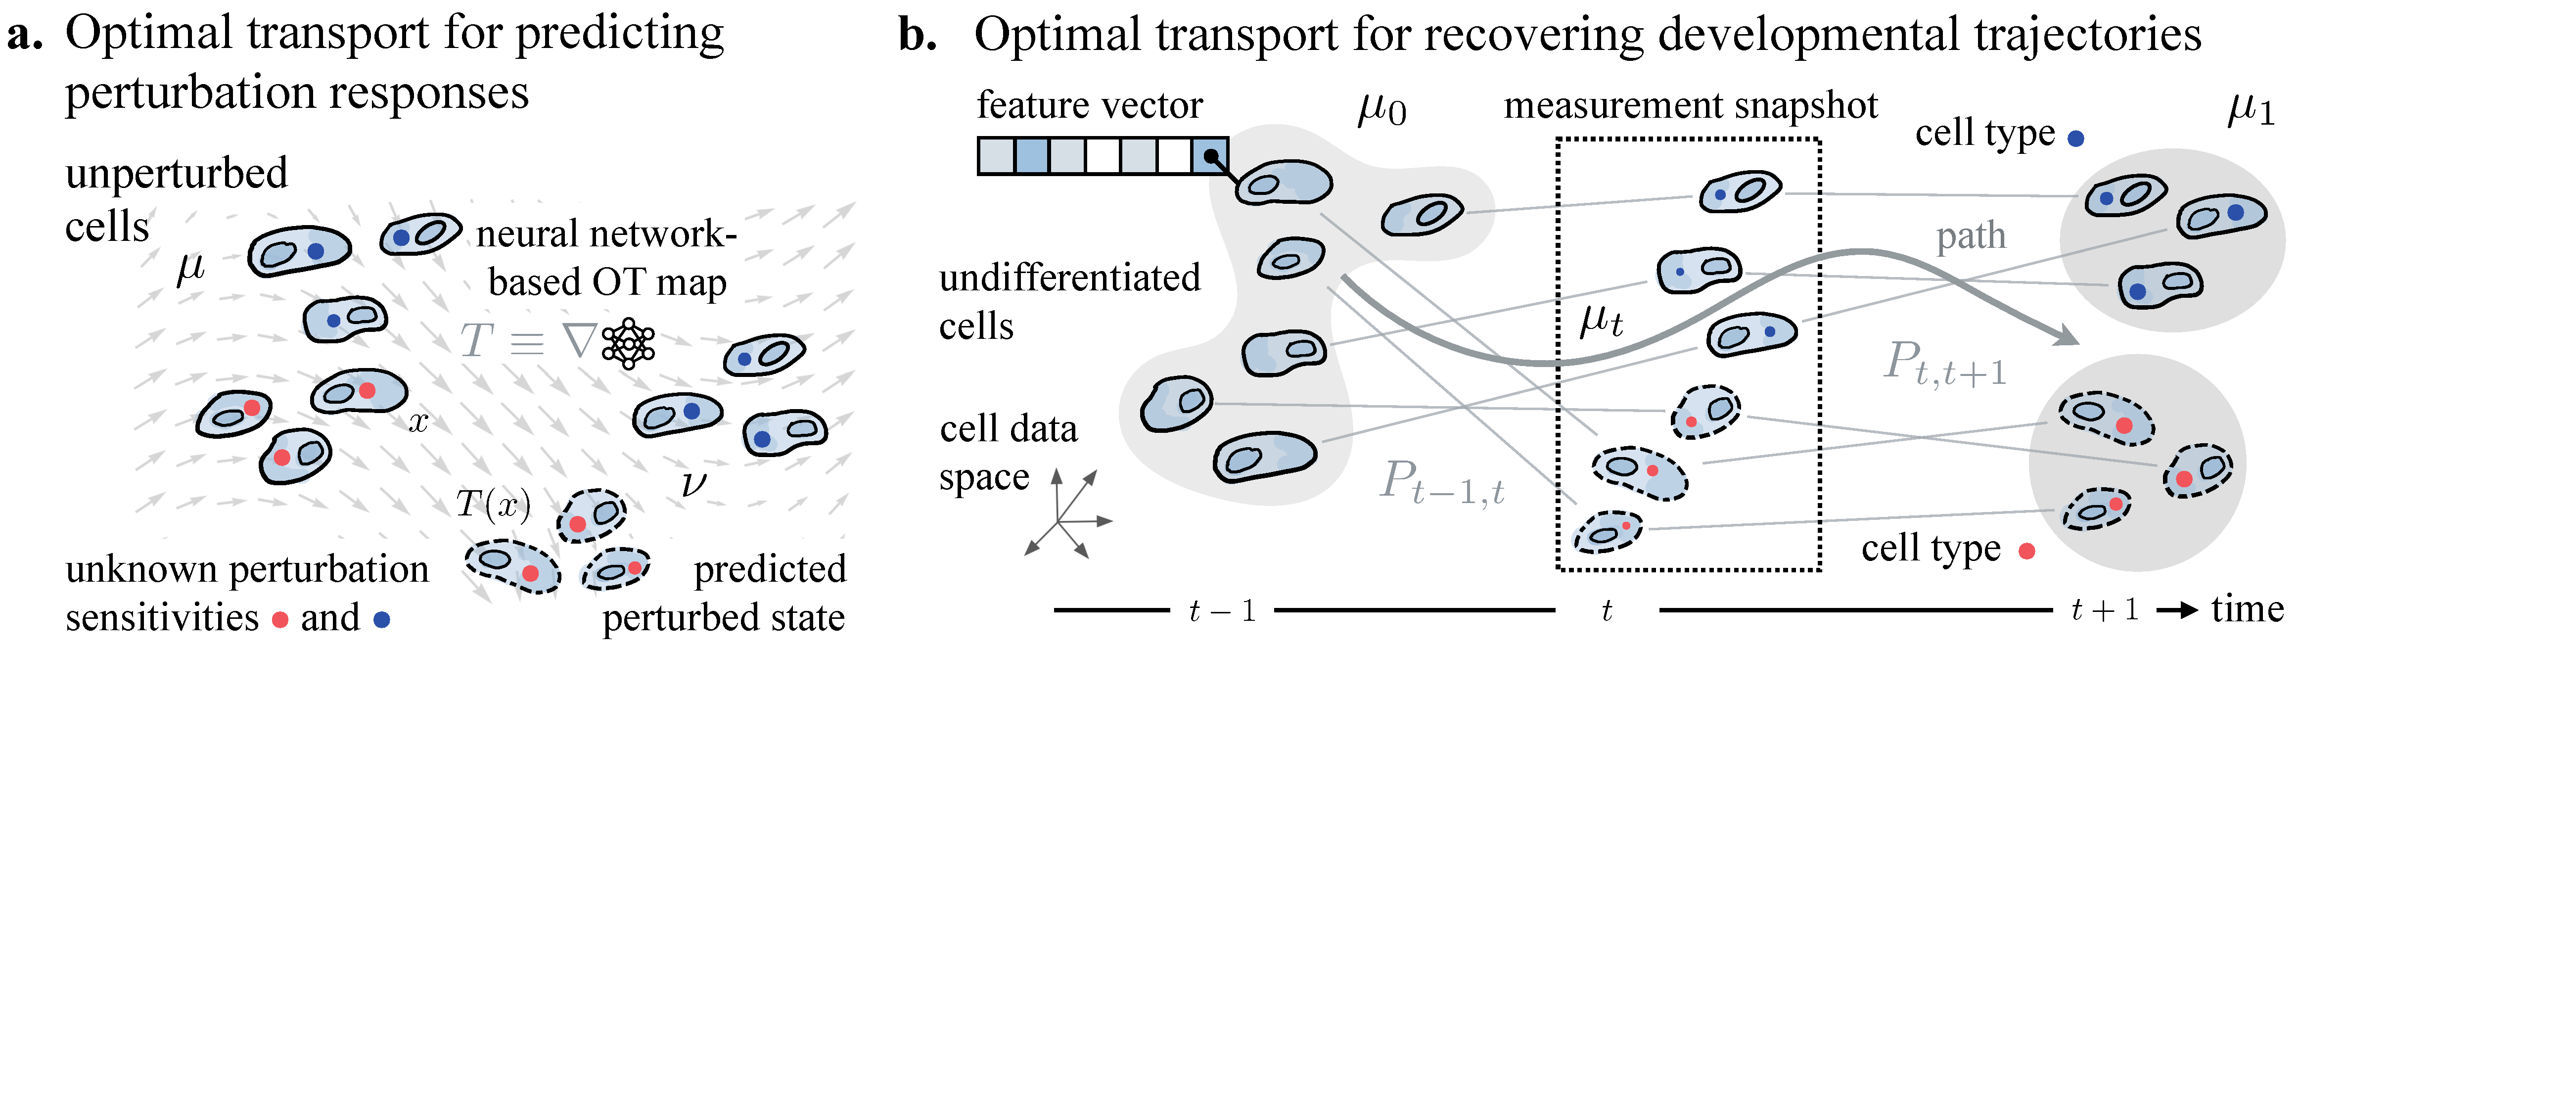
\includegraphics[width=\textwidth]{figures/fig_bio_problems.pdf}
  \caption{\textbf{Overview on different dynamical processes in biomedicine.} \textbf{a.} ... \textbf{b.} ...}	
  \label{fig:bio_problems}
\end{figure}


\chapter{Optimal Transport for Dynamical Systems}
\label{cha:theory_background}

\dictum[Elinor Ostrom, \textit{Governing the Commons} (1990)]{%
  The power of a theory is exactly proportional to the diversity of situations it can explain.}%
\vskip 1em


Optimal transport theory~\citep{santambrogio2015optimal} is a core element of the machine learning toolbox and has become within a few years the go-to framework to analyze, model, and solve an ever-increasing variety of tasks involving probability measures. This is best exemplified by its increasing importance to fitting generative models, where the goal is to learn a map~\citep{arjovsky2017wasserstein, genevay2018learning, salimans2018improving}, or more generally a diffusion \citep{song2020score, de2021diffusion} to morph a simple measure (e.g., Gaussian) onto a data distribution of interest (e.g., images). This is also apparent in the many applications that use OT to align probability measures that have since arisen, e.g., to transfer label knowledge between datasets~\citep{flamary2016optimal, singh2020model}, to analyze sampling schemes~\citep{dalalyan2017theoretical}, or study population trajectories~\citep{schiebinger2019optimal, bunne2021learning}.

In this chapter, we primarily cast light on the static and dynamic formulation of optimal transport, and simultaneously establish their theoretical nexus by recalling its mathematical history from \citet{monge1781histoire} and \citet{kantorovich1942transfer} to modern Fields Medal winners \citet{villani2009optimal}, \citeauthor{figalli2010optimal}, and Abel Prize recipient \citet{caffarelli1990interior} in order to provide a solid foundation for the discussion ahead.


\section{Static Optimal Transport} \label{sec:background_ot_static}

\looseness -1 Optimal transport takes dual roles as it induces a mathematically well-characterized distance measure between distributions as well as provides a geometry-based approach to realize mappings between two probability distributions.
In this section, we introduce the mathematical foundations of the \textbf{static} OT problem. Further, we will provide an extended analysis of the \citeauthor{monge1781histoire} map, which provides an actionable way to flow from one probability distribution onto another.
We conclude with a complete proof of the celebrated \citeauthor{brenier1987decomposition} theorem. This quintessential result and its particularization to translation-invariant costs lays the foundation of the flurry of neural approaches proposed in the literature. This includes modeling Monge maps as gradients of convex functions parameterized through convex neural networks \citep{amos2017input, huang2021convex, makkuva2020optimal, korotin2021neural, lubeck2022neural, bunne2022supervised}, i.e., approaches that are a direct consequence of the \citeauthor{brenier1987decomposition} theorem and subject of this thesis, regularizers \citep{uscidda2023monge}, amortized optimization \citep{amos2022amortizing, amos2022meta}, or entropic maps \citep{pooladian2021entropic, pooladian2023minimax, divol2022optimal, cuturi2023monge}.

\begin{figure}[t]
  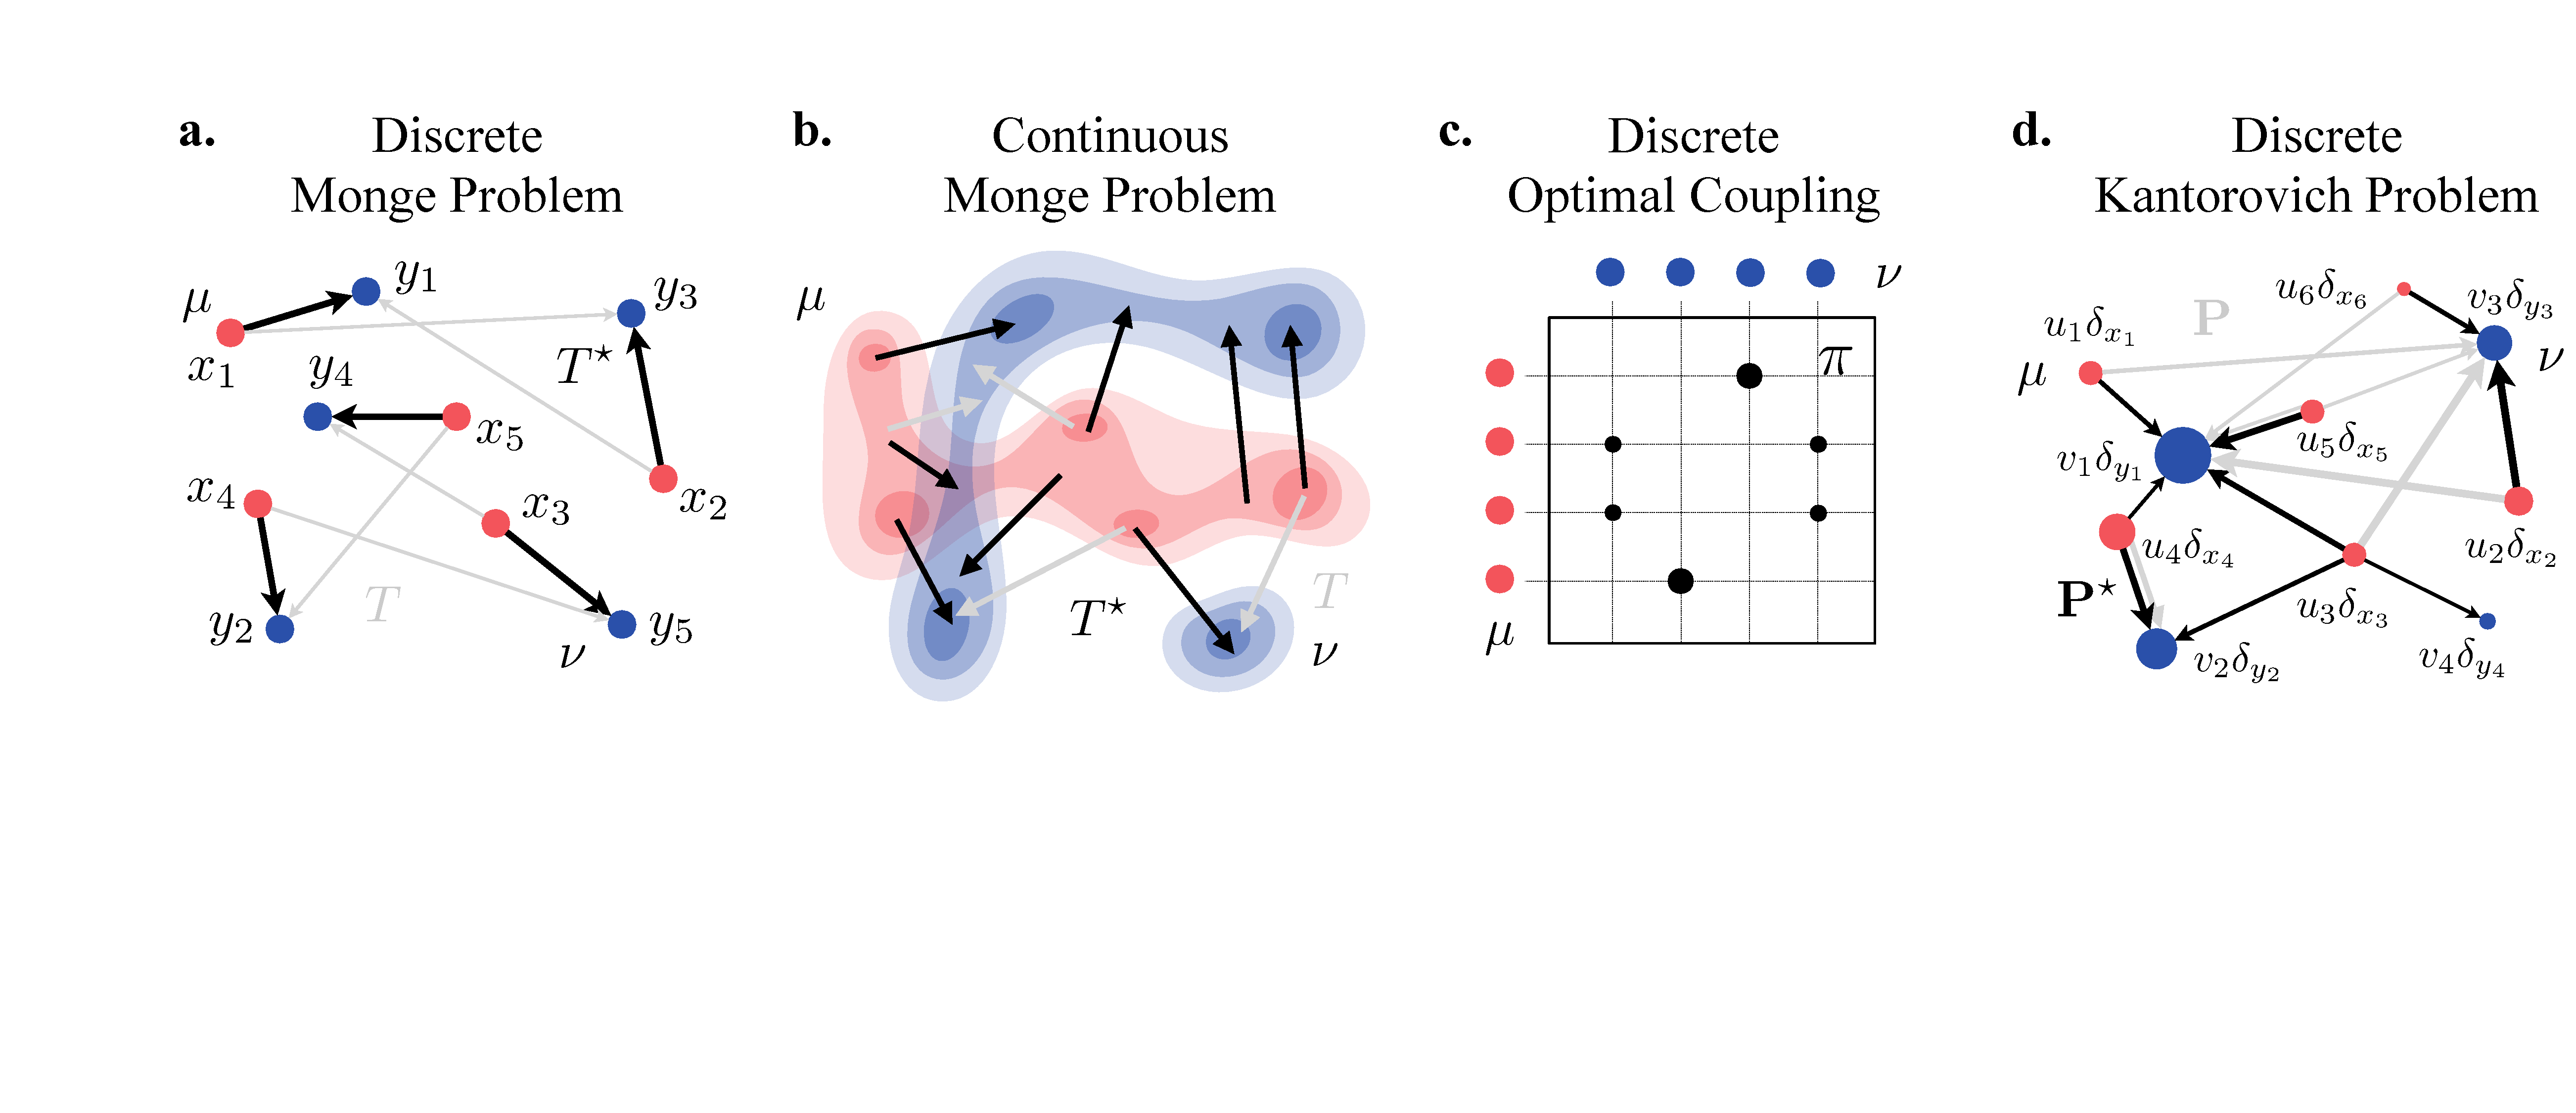
\includegraphics[width=\textwidth]{figures/fig_ot_background.pdf}
  \caption{\textbf{Overview on different formulations of the static OT problem for discrete and continuous measures.} Monge map for \textbf{a.} discrete and \textbf{b.} continuous measures $\mu, \nu$. The optimal map $T^\star$ minimizes \eqref{eq:monge}. \textbf{c.} Optimal coupling $\pi$ \eqref{eq:kantorovich} for discrete measures $\mu$ and $\nu$. \textbf{d.} Mass splitting principle of the Kantorovich relaxation for discrete measures $\mu$ and $\nu$ of the optimal transport plan $\bP^\star$ and a non-optimal plan $\bP$. Figure adapted from \citet{peyre2019computational}.}	
  \label{fig:ot_principles}
\end{figure}

\subsection{Monge Problem} \label{sec:background_monge}

In the 18th century "M{\'e}moire sur la th{\'e}orie des d{\'e}blais et des remblais", Gaspard Monge sets out to solve what is now known as the \citeauthor{monge1781histoire} problem, posing a seemingly simple, yet fundamentally complex question: Given two quantities of mass located at two different sites, what is the most efficient way to transport one into the other?
In more formal terms, provided with two measures $\mu, \nu\in \mathcal{P}(\mathbb{R}^d)$, here restricted to measures supported on $\mathbb{R}^d$, \citeauthor{monge1781histoire}'s initial approach was to find a map $T$ that pushes one mass onto the other in a way that minimizes the total cost of transport.
Given a measurable const function $c: \mathcal{X} \times \mathcal{Y} \rightarrow \mathbb{R}$, the \citeauthor{monge1781histoire} problem then reads
\begin{equation}\label{eq:monge}
T^\star := \arg\inf_{T\sharp\mu=\nu}\int_{\mathbb{R}^d} c(x, T(x)) d\mu(x)\,.
\end{equation}
For two discrete measures $\mu=\sum_{i=1}^n u_i \delta_{x_{i}}, \nu=\sum_{j=1}^m v_j \delta_{y_{j}}$, it seeks a transport map $T: \mathcal{X} \rightarrow \mathcal{Y}$ associating each source point $x_i$ to a target point $y_j$ (see \cref{fig:ot_principles}a for the discrete and \cref{fig:ot_principles}b for the continuous setting).
... % TODO: Add more butter.
The existence of $T^\star$ is guaranteed under fairly general conditions \citep[Theorem 1.22]{santambrogio2015optimal}, which require that $\mu$ and $\nu$ have finite $\ell_2$ norm, and that $\mu$ puts no mass on $(d-1)$ surfaces of class $\mathcal{C}_2$.


\subsection{Kantorovich Relaxation} \label{sec:background_kantorovich}

It was not until the 20th century, however, that the concept found a more tractable development. In \citeyear{kantorovich1942transfer}, Leonid \citeauthor{kantorovich1942transfer} provided a relaxation to this non-convex and difficult-to-solve problem.
Instead of the deterministic matching proposed by \citeauthor{monge1781histoire}, Kantorovich considered probabilistic correspondences that allow for transportation of mass from a single source point to various target points (mass splitting), resulting in the problem formulation
\begin{equation} \label{eq:kantorovich}
    W(\mu, \nu) = \inf_{\pi\in \Pi(\mu,\nu)}\iint c(x, y) \pi(dx, dy),
\end{equation}
where $\Pi(\mu, \nu) \defeq \left\{\pi \in \gP(\mathcal{X} \times \mathcal{Y}): P_{\gX \sharp} \pi=\mu \, \text { and } \, P_{\gY \sharp} \pi=\nu\right\}$ is the set of couplings on $\mathbb{R}^d\times\mathbb{R}^d$ with respective marginals $\mu, \nu$. Given the optimal transport coupling $\pi$, the resulting distance $W(\mu, \nu)$ between $\mu$ and $\nu$ is known as the Wasserstein distance.
A visualization of the discrete setting is provided in \cref{fig:ot_principles}c.

For his work, \citeauthor{kantorovich1942transfer} received the Nobel Prize in economics. The connections of \acrshort{OT} to basic questions in economy becomes clear when interpreting $\mu$ as a density of resource units, and $\nu$ a density of factories, where the coupling $\pi$ denotes the optimal transportation plan of distributing resources to factories.

% TODO: Add general formulation of regularized OT problem.
When instantiated on finite discrete measures, such as $\mu=\sum_{i=1}^n u_i\delta_{x_i}$ and $\nu=\sum_{j=1}^m v_j\delta_{y_j}$, this problem translates to a linear program, which can be regularized using an entropy term~\citep{cuturi2013sinkhorn,peyre2019computational}. For $\varepsilon\geq0$, set 
\begin{equation} \label{eq:reg-ot}
\We(\mu,\nu) \defeq \min_{\bP\in U(u, v)} \dotp{\bP}{[c(x_i, y_j)]_{ij}}  \,-\varepsilon H(\bP),
\end{equation}
where the discrete entropy of transportation plan $\bP$ is defined as $H(\bP) \defeq -\sum_{ij} \bP_{ij} (\log \bP_{ij} - 1)$ and the polytope $U(u, v)$ is the set of $n\times m$ matrices $\{\bP\in\mathbb{R}^{n \times m}_+, \bP\mathbf{1}_m =u, \bP^\top\mathbf{1}_n=v\}$. 
Notice that the definition above reduces to the usual Wasserstein distance when $\varepsilon=0$. Setting $\varepsilon>0$ yields a faster and differentiable proxy to approximate $W_{0}$, but introduces a bias, since $\We(\mu,\mu)\ne 0$ in general.
Thus, regularizing objective \eqref{eq:kantorovich} with an entropy term results in a significantly more efficient optimization \citep{cuturi2013sinkhorn} and differentiability w.r.t. its inputs. As a consequence, \eqref{eq:reg-ot} is commonly used as a loss function in machine learning applications, e.g., for structured prediction \citep{frogner2015learning,janati2020multi} or generative model fitting \citep{arjovsky2017wasserstein, salimans2018improving, genevay2018learning}.


\subsection{Kantorovich Duality} \label{sec:background_dual}

The Kantorovich formulation \eqref{eq:kantorovich} is a \emph{convex} problem on $\gP(\mathcal{X} \times \mathcal{Y})$ and thus admits a dual formulation introduced by \citet{kantorovich1942transfer}, i.e., a constrained concave maximization problem defined as
\begin{equation} \label{eq:kantorovich-dual}
    W(\mu, \nu)=\sup _{(f, g) \in \Phi_{c}} \int f \mathrm{~d} \mu+\int g \mathrm{~d} v,
\end{equation}
\looseness -1 where the set of admissible dual potentials is given by $\Phi_c \defeq \{(f, g) \in L^{1}(\mu) \times L^{1}(\nu): f(x)+g(y) \leq c(x,y)$, $\forall(x, y) d\mu \otimes d\nu \text{ a.e.}\}$.
$(f, g)$ is thus a pair of continuous functions, often referred to as \emph{Kantorovich potentials}.
An informal interpretation of \eqref{eq:kantorovich-dual} was provided by \citet{caffarelli2003monge}, revisiting the connection of \acrshort{OT} to economics: 
A logistics company is concerned with transporting products from each resource unit $x$ to a factory $y$. The transportation company thereby charges $f(x)$ for loading resources at point $x$ and $g(y)$ of unloading it at destination $y$, but is constrained to charge $f(x)+g(y) \le c(x,y)$. In order to arrange prizes $f$ and $g$ that increase profit, they thus maximize objective \eqref{eq:kantorovich-dual}.

% TODO: Provide a better transition. 
Beyond, using the notion of $c$-transforms, i.e.,
\begin{equation}
	\tag{$c$-transform}
	\forall y \in \mathcal{Y}, \quad f^c(y) \defeq \inf _{x \in \mathcal{X}} c(x, y)-f(x) \,,
\end{equation}
we can reduce \eqref{eq:kantorovich-dual} to a single potential: Assume we keep dual potential $f$ fixed, the potential $g$ needs to satisfy for all $x, y$
\begin{align*}
	f(x) + &g(y) \le c(x, y)\,,
	\forall y \in \mathcal{Y}, \quad  &g(t) \ge f^c(y) \defeq \inf _{x \in \mathcal{X}} c(x, y) - f(x)\,,
\end{align*}
resulting in the semi-dual
\begin{equation}\label{eq:semi-dual}
\arg\!\!\max_{f\, c\text{-concave}} \int f \textrm{d}\mu + \int f^c\textrm{d}\nu\,.
\end{equation}

\paragraph{Euclidean case.} For the cost $c(x, y) = \norm{x-y}^2$ in $\gX = \gY = \mathbb{R}^d$, one can replace the constraint of \eqref{eq:kantorovich-dual} using the Legendre-Fenchel transform
\begin{equation} \label{eq:legendre_fenchel}
	\tag{Legendre-Fenchel transform}
	\forall y, \quad g(y) \geq f^*(y) \defeq \sup _x \langle x, y\rangle-f(x)\,,
\end{equation}
where $f^*$ is the convex conjugate of $f$ and a convex function (as a supremum of linear functions). Then, the semi-dual in the Euclidean setting reads
\begin{equation} \label{eq:dual-cvx}
	\arg\!\!\min_{f\, \text{convex}} \int f \textrm{d}\mu + \int f^*\textrm{d}\nu\,.
\end{equation}
Further, following the double convexification trick as outlined in \citet[Lemma 2.10]{villani2021topics}, we see that applying the \ref{eq:legendre_fenchel} twice results in function pair $(f^{**},f^{*})$ and thus, as each of them is defined as the supremum of a family of linear functions, an optimization problem over two convex lower semi-continuous functions.

\subsection{Brenier Theorem} \label{sec:background_brenier}

Problem \eqref{eq:kantorovich-dual} allows us to characterize optimal transport plans that emerge as the solution to the Kantorovich optimal transportation problem \eqref{eq:kantorovich} and show sufficient conditions for the existence of optimal transport maps.
Although a large part of optimal transport theory can be developed in a general framework as above, for the rest of the section, we will resort to the case $c(x, y):=\|x-y\|^2$ on $\mathbb{R}^d \times \mathbb{R}^d$. Generalizations to other cost functions are possible but with an additional notational burden\footnote{For example it is possible to show the existence of optimal transport maps for strictly convex and superlinear cost functions, and characterize them in terms of $c$-superdifferentials of $c$-convex functions.}.
In the following, we will give a characterization of optimal transport plans \citep{knott1984optimal}:

\begin{theorem}[Knott-Smith Optimality Criterion]
	...
\end{theorem}
\begin{proof}
	For the complete proof, see \citet[Proof of Theorem 2.12]{villani2021topics}.
\end{proof}
In convex analysis this property is called cyclical monotonicity.

The next result specifically gives conditions sufficient for the existence of transport maps.
The celebrated \citeauthor{brenier1987decomposition} theorem \citeyearpar{brenier1987decomposition} establishes for the special case of the Euclidean distance the equivalence of the Monge \eqref{eq:monge} and Kantorovich formulation  \eqref{eq:kantorovich}, the uniqueness of the optimal coupling $\pi$, and states that there must exist a unique (up to the addition of a constant) potential $f^\star:\mathbb{R}^d\rightarrow \mathbb{R}$ such that $T^\star = \nabla f^\star$. 
This theorem has far-reaching implications: It is sufficient, when seeking optimal transport maps, to restrict the computational effort to seek a "good" convex potential, such that its gradient pushes $\mu$ towards $\nu$. 
More formally:

\begin{theorem}[Brenier Theorem] \label{thm:brenier}
	In the setting where both $\mathcal{X}$ and $\mathcal{Y}$ are equal to $\mathbb{R}^d$, and the cost function $c(x, y) = norm{x-y}^2$ is employed, and at least one of the two input measures $\mu$ possesses a density $\rho_\mu$ in relation to the Lebesgue measure, then there exists a unique optimal solution $\pi$ in the Kantorovich formulation \eqref{eq:kantorovich}.
	This solution is exclusively supported on the graph $(x, T(x))$ of Monge map $T: \mathbb{R}^d \rightarrow \mathbb{R}^d$.
	In other terms, we can express $\pi$ as $(\operatorname{Id}, T)_{\sharp} \alpha$, meaning that for any function $h$ belonging to the set $\forall h \in \mathcal{C}(\mathcal{X} \times \mathcal{Y})$, the following equality holds
	$$
	\quad \int_{\mathcal{X} \times \mathcal{Y}} h(x, y) \mathrm{d} \pi(x, y)=\int_{\mathcal{X}} h(x, T(x)) \mathrm{d} \mu(x).
	$$
Moreover, this map $T$ is uniquely determined by the gradient of a convex function $\psi$, denoted as $T(x)=\nabla \psi(x)$. The function $\psi$ is the unique convex function, up to an additional constant, for which $(\nabla \psi)_{\sharp} \mu=\nu$. We can establish a relationship between this convex function $\psi$ and the dual potential $f$ that solves \eqref{eq:kantorovich-dual} by expressing $\psi(x)$ as $\frac{|x|^2}{2}-f(x)$.
\end{theorem}
\begin{proof}
	...
\end{proof}
...
\begin{corollary}
	Under the assumption of \cref{thm:brenier}, $\nabla \psi$ is the unique solution to the Monge transportation problem \eqref{eq:monge}, i.e.,
	\begin{equation}
		\int_{\mathbb{R}^d} \norm{x-\nabla \psi(x)}^2 \mathrm{d}\mu(x) = \inf_{T_\sharp \mu = \nu} \int_{\mathbb{R}^d}\norm{x - T(x)}^2 \mathrm{d}\mu(x).
	\end{equation}
\end{corollary}
This result has been exploited to propose neural OT solvers ~\citep{makkuva2020optimal, korotin2021wasserstein, bunne2022proximal, alvarez2021optimizing, mokrov2021large} and  will recurrently permeate this thesis, proving its essential nature in multiple instances and modern developments of optimal transport.
In particular, it presents an elegant way to solve the Monge problem in a geometric sense and has profound implications for the dynamic version of the problem, which we will study next.


\section{Dynamic Optimal Transport} \label{sec:background_ot_dynamic}

\begin{figure}[t]
  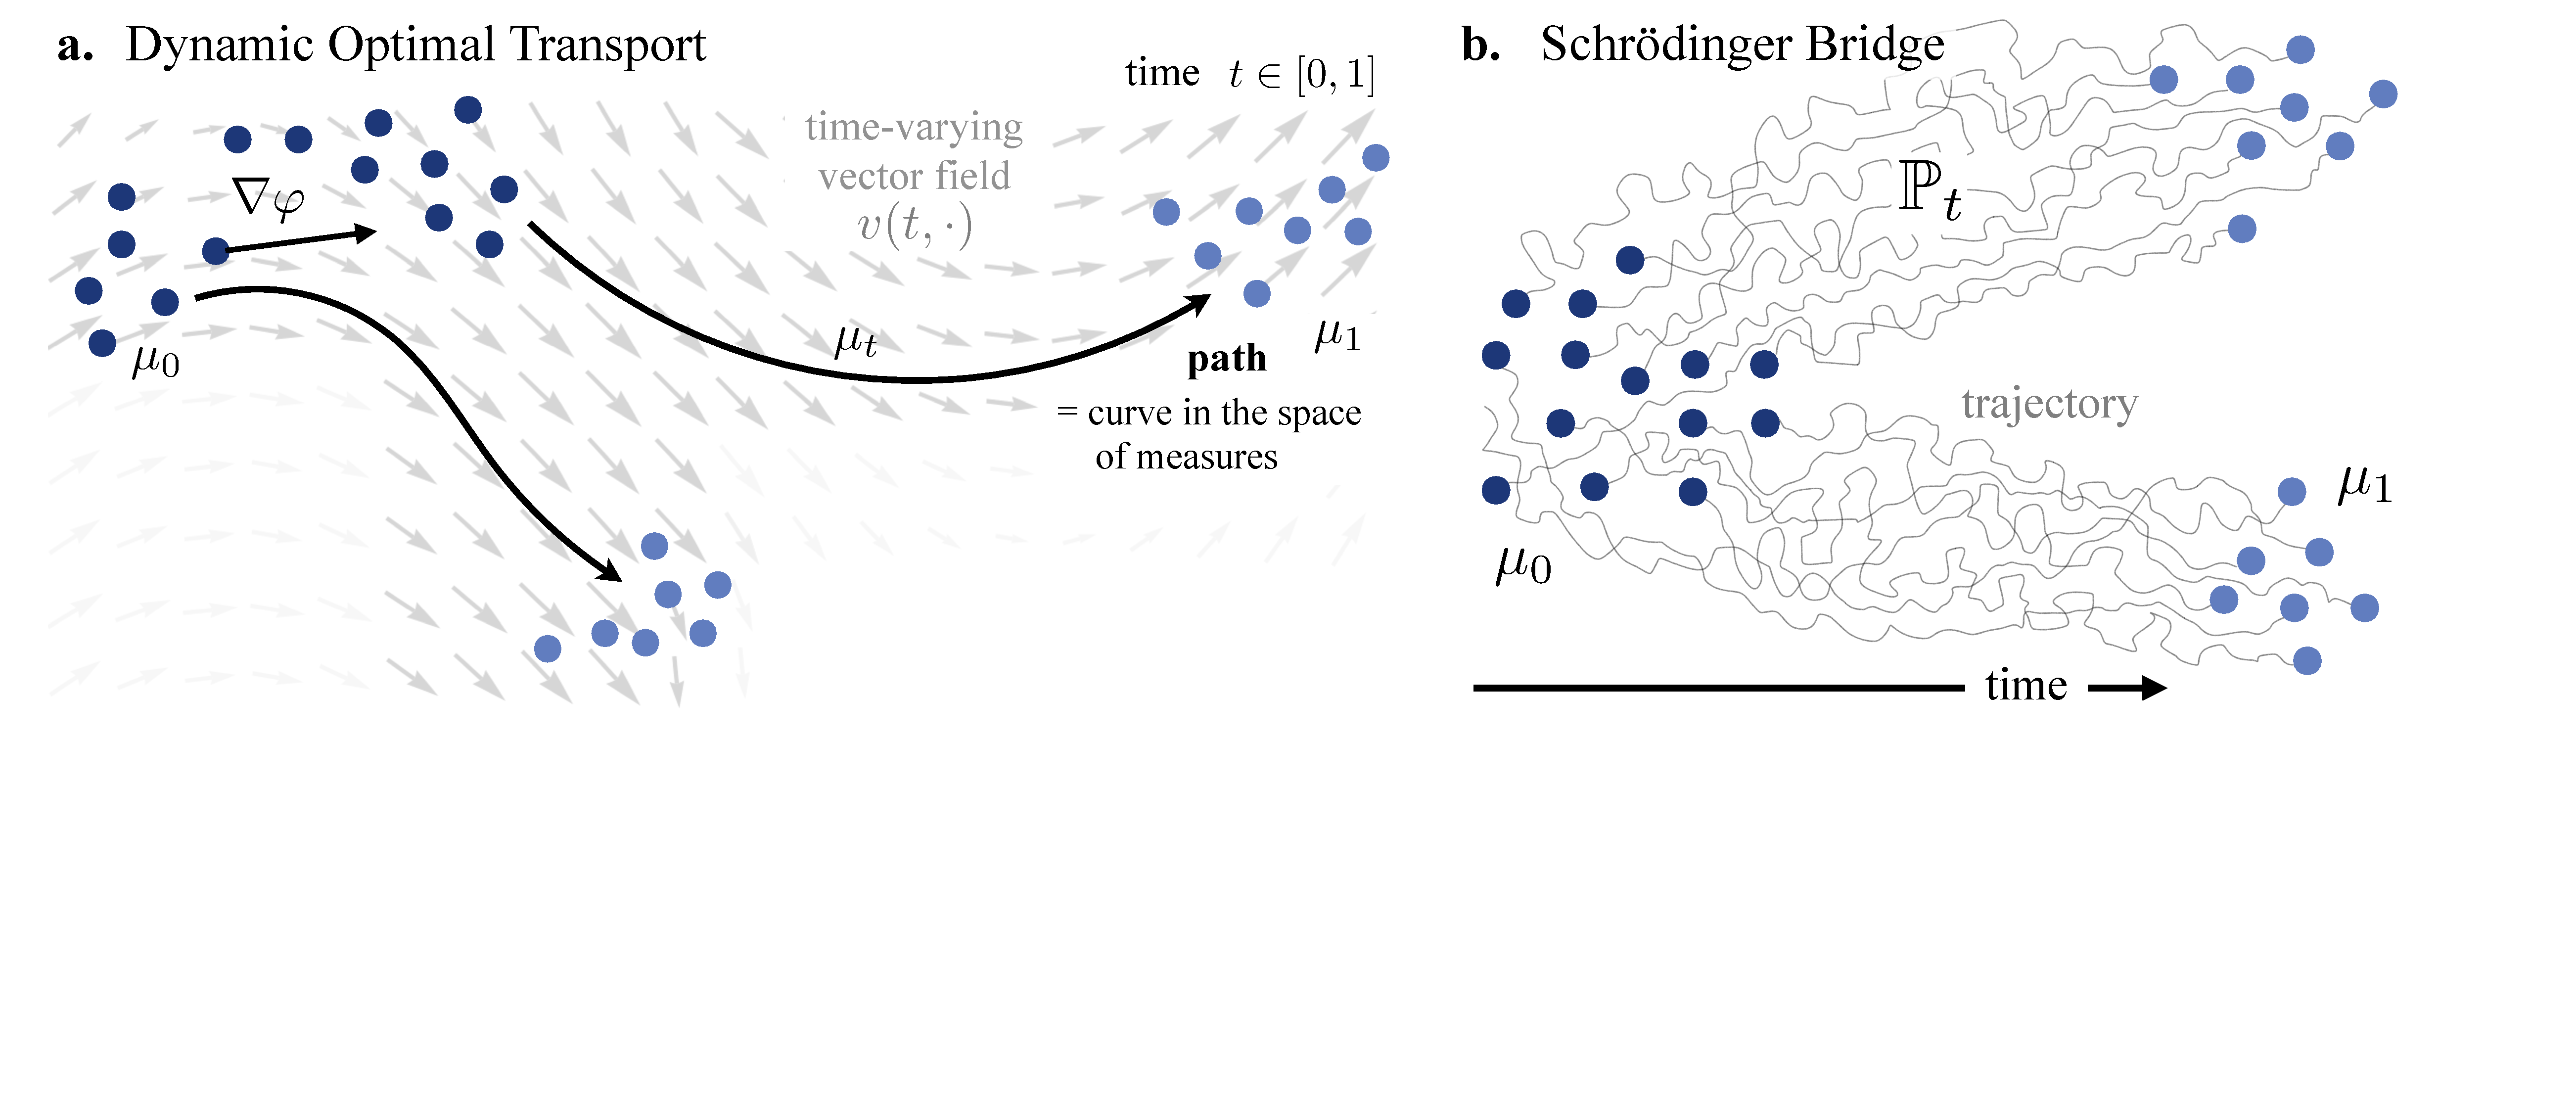
\includegraphics[width=\textwidth]{figures/fig_dynamic_ot_background.pdf}
  \caption{\textbf{Overview on different formulations of the dynamic OT problem.} \textbf{a.} ... \textbf{b.} ...}	
  \label{fig:dynamic_ot_background}
\end{figure}

We have hitherto engaged with the \emph{static} \acrlong{OT} problem, establishing a solid foundation upon which to build more intricate dynamic formulations. In fact, the roots of these dynamic formulations are embedded within the static \acrshort{OT} framework: As posited by \citet{benamou2000computational}, the dynamic formulation "was already implicitly contained in the original problem addressed by \citeauthor{monge1781histoire}", where "eliminating the time variable was just a clever way of reducing the dimension of the problem." When reintroducing time in the dynamic version, the optimal transport map becomes a time-dependent flow capable of describing the evolution of a measure over time.

In this section, we will cover several perspectives and frameworks of the \textbf{dynamic} \acrshort{OT} problem: As mentioned earlier, \citeauthor{brenier1987decomposition} theorem thereby forms a critical bridge that connects the static and dynamic formulation, perpetuated in the Monge-Amp{\`e}re equation.
Further, \citet*{benamou2000computational} introduce how the dynamic point of view offers an alternate and intuitive interpretation of optimal transport with links to fluid dynamics. The resulting framework surprisingly leads to a convex optimization problem that can be parameterized through normalizing flows \citep{tong2020trajectorynet}.
We further highlight the connections of \acrshort{OT} to \acrshortpl{PDE} such as Fokker-Planck-like equations through the \citeauthor*{jordan1998variational} scheme.
Lastly, moving beyond PDEs and taking a stochastic control perspective, we will introduce the notion of the Schr\"odinger bridge problem.


\subsection{Monge-Amp{\`e}re Equation} \label{sec:background_monge_ampere}

% Caffarelli's regularity theorems from the 1990s represented a major breakthrough in our understanding of the Monge-Amp{\`e}re equation, a highly nonlinear, quintessential partial differential equation, that for instance is used to construct surfaces of prescribed Gaussian curvature. Important existence results were established by Alexandrov, and earlier central properties had been shown by Caffarelli in collaboration with Nirenberg and Spruck, with further key contributions by Evans and Krylov. Caffarelli however closed the gap in our understanding of singularities by proving that the explicitly known examples of singular solutions are the only ones.

% Caffarelli has, together with collaborators, applied these results to the Monge-Kantorovich optimal mass transportation problem, based on previous work by Brenier. Caffarelli and Vasseur gave deep regularity results for the quasi-geostrophic equation in part by applying the exceptionally influential paper by Caffarelli and Silvestre on the fractional Laplacian.
As a direct consequence of \cref{thm:brenier}, if $T(x) = \nabla \psi(x)$, $\psi$ being smooth and strictly convex, and $\mu$ and $\nu$ absolutely continuous with densities $\rho_\mu$ and $\rho_\nu$, we can express $T_\sharp \mu = \nu$ in a nonlinear \acrfull{PDE} form. More concretely, $\psi$ is a solution of the Monge-Amp{\`e}re equation that reads
\begin{equation} \label{eq:monge_ampere}
	\operatorname{det}\left(\partial^2 \psi(x)\right) \rho_\nu(\nabla \psi(x))=\rho_\mu(x),
\end{equation}
where $\partial^2 \psi(x) \in \mathbb{R}^{d \times d}$ is the Hessian of $\psi$, describing the continuous evolution from $\mu$ to $\nu$.
First studied by \citeauthor{monge1781histoire} in \citeyear{monge1781histoire} and later by \citeauthor{ampere1819memoire} in \citeyear{ampere1819memoire}, this nonlinear partial differential equation arises in several problems from analysis to geometry, for example, in the Weyl and Minkowski problems in differential geometry of surfaces. 
The regularity of the solutions of \eqref{eq:monge_ampere}, with implications on regularity results of the optimal transport map $T$, has been subject of a series of works by \citeauthor{caffarelli1990interior} in the \citeyear{caffarelli1990interior}s, for which he was awarded the Abel Prize in 2023, as well as more recently by \citeauthor{figalli2017monge}, recognized with the Fields Medal in 2023.


\subsection{Benamou-Brenier Formulation} \label{sec:background_benamou_brenier}

Avoiding solving \eqref{eq:monge_ampere} directly, \citet{benamou2000computational} introduce an alternative numerical framework by connecting the optimal mass transfer problem to continuum mechanic frameworks.
Deviating from the previous notation of $(\mu, \nu)$, in the following sections we study the dynamic problem via the evolution from measure $\mu_0$ at time $t=0$ to $\mu_1$ at $t=1$. The solution of \eqref{eq:kantorovich} then coincides with finding the minimal path $(\mu_t)_{t=0}^1$, or more concretely, a curve in the space of measures, minimizing a total length.  
Such path $\mu_t$ can be described through a vector field $v_t$ which moves particles around, satisfying the continuity equation in fluid dynamics or conservation of mass formula
\begin{equation} \label{eq:continuity_equation}
	\frac{\partial \mu_t}{\partial t}+\nabla\left(\mu_t v_t\right)= 0, \qquad \mu_{t=0}=\mu_0, \mu_{t=1}=\mu_1\,,
\end{equation}
where the vector field $v_t$ denotes the speed and $\mu_t v_t = J_t$ corresponds to the momentum.
Reformulating the optimal transportation problem in a differential way, an "Eulerian" formulation inspired by fluid mechanics, will be crucial for the subsequent study of dynamical problems.
Every curve $\mu_t$ describing the evolution of the measure over time can thereby be interpreted as the fluid flow along a family of vector fields. We are searching for the vector field $v_t$ that (i.) that satisfies the conservation of mass \eqref{eq:continuity_equation}, and (ii.) minimized the path length.
The infinitesimal length of such a vector field can be computed via 
\begin{equation} \label{eq:vector_field_length}
	\left\|v_t\right\|_{\ell^2\left(\mu_t\right)}=\left(\int_{\mathbb{R}^d}\left\|v(t, x)\right\|^2 \mathrm{~d} \mu_t(x)\right)^{1 / 2}.
\end{equation}
resulting, in the case of $\gX = \gY = \mathbb{R}^d$ and $c(x, y)=\|x-y\|^2$, in the minimal-path reformulation of \eqref{eq:kantorovich}
\begin{align}  \label{eq:benamou_brenier}
	W\left(\mu_0, \mu_1\right)=& \inf _{(\mu_t, v)} \int_0^1 \int_{\mathbb{R}^n}\frac{1}{2}\norm{v(t, x)}^2 d\mu_t(x) d t \\
	& \nonumber \frac{\partial \mu_t}{\partial t}+\nabla \cdot(v \mu_t)=0 \\
	& \nonumber \mu_{t=0}=\mu_0, \mu_{t=1}=\mu_1\, .
\end{align}
Taking the perspective of fluid dynamics, \eqref{eq:vector_field_length} can also be interpreted as the \emph{kinetic energy} of the particles. The Benamou-Brenier formulation \eqref{eq:benamou_brenier} then selects the vector field $v_t$ that minimizes the total efforts or the total kinetic energy one has to spend in order to move particles around according to the vector field $v_t$.

\paragraph{Euclidean case.} A particular important case occurs again in the Euclidean setting, i.e., for cost $c(x, y) = \norm{x-y}^2$ in $\gX = \gY = \mathbb{R}^d$. The solution of the time-dependent OT problem \eqref{eq:benamou_brenier} then coincides with \citeauthor{mccann1997convexity}'s displacement interpolation between two measures.
Reciting \cref{thm:brenier}, with $T = \nabla \psi$, $\mu_t$ is equal to \citeauthor{mccann1997convexity}'s interpolation between $\mu_0$ and $\mu_1$ given by
\begin{equation} \label{eq:mccann_interpolation}
	\mu_t = [(1-t) I+t \nabla \psi]_\sharp \mu_0 = [(1-t) I+t T]_\sharp \mu_0\,.
\end{equation}
Despite their simplicity, this concept possesses remarkable applications beyond the realm of optimal transport \citep{bonneel2011displacement}. In particular, its interpretation as a geodesic formula in Riemannian geometry is thoroughly discussed in \citet{gangbo1996geometry}, and serves as a pivotal link to the subsequent discussion.


\subsection{Jordan-Kinderlehrer-Otto Flows} \label{sec:background_jko}

The time-dependent Benamou-Brenier formulation \eqref{eq:benamou_brenier} not only provides us with a more complete description of optimal transport, but also the discovery that the resulting path $(\mu_t)_{t=0}^1$ may be seen as a constant-speed geodesic interpolating between population $\mu_0$ and $\mu_1$ in the space of measures, i.e., a Wasserstein geodesic.
Following \citet{otto2001geometry} on the calculus of optimal transport (\citeauthor{otto2001geometry} calculus), a large class of PDEs may then be viewed as gradient flows on the Wasserstein space \citep{jordan1998variational}.
A gradient flow is thereby a curve following the direction of steepest descent of a function $F$.

\paragraph{Euclidean case.} Considering the evolution of a vector $x$ over time in the Euclidean space, with $F$ being smooth, this can be realized through the standard gradient descent (forward) scheme
\begin{equation*}
	x_{t+1} \defeq x_{t}-\tau \nabla F\left(x_{t}\right),
\end{equation*}
where $\tau$ is the step size. For non-smooth functions, on can resort to a proximal (backward) scheme, i.e.,
\begin{equation*}
	x_{t+1} \defeq \operatorname{Prox}_{\tau F}^{\|\cdot\|}\left(x_{t}\right) \defeq \arg\!\min_x \frac{1}{2}\left\| x-x_t\right\|^2+\tau F(x).
\end{equation*}

\paragraph{Wasserstein case.} When studying the evolution of measure $\mu_t$ over time, we will resort to optimal transport metrics the $\ell_2$-norm $\norm{\cdot}$.
Considering a functionals $F$ taking a measure as input, a gradient flow of $\mu$ w.r.t. to $F$ 
\begin{equation}
	\mu_{t+1} \defeq \arg\!\min_\mu W(\mu, \mu_t)^2+\tau F(\mu).
\end{equation}
...

In recent works, \acrshort{JKO} flows have found application in inferring the evolution of populations over time, crucial in many scientific disciplines when for instance, observing a population of cells in biology \citep{bunne2022proximal, alvarez2021optimizing, mokrov2021large, benamou2016augmented}.

\subsection{Stochastic Control Perspective} \label{sec:background_control}

Benamou-Brenier motivated the introduction of the dynamic optimal transport problem from a perspective of fluid dynamics.
As we shall see, both the OT problem \eqref{eq:kantorovich} and its regularized version \eqref{eq:reg-ot} can be viewed as stochastic \textit{optimal control} problems.
... % why do we want this?
Control theory at the heart is concerned with finding optimal policies for dynamic systems subject to constraints. Despite wide-ranging progress on both the theory and applications, deploying control theory to large-scale and often unknown systems remains a grand challenge.
As we will explore in the following, stochastic optimal control problems to regulate dynamic systems emerge from the theory of optimal transport \citep{santambrogio2015optimal} that provides geometric variational framework for studying flows of distributions on metric spaces \citep{chen2021optimal}.
These theoretical concepts build the foundation of recently developed deep learning architectures employed as generative models \citep{song2020score, de2021diffusion} or for studying the evolution of dynamical systems over time \citep{chen2021likelihood, bunne2022proximal, vargas2021solving}.
Further, celebrated control principles such as the Pontryagin maximum principle have been emphasized repeatedly in neural ordinary equation \citep{chen2018neural} and stochastic differential equation works \citep{jia2019neural}.

\subsubsection*{... on Optimal Transport} \label{sec:background_control_ot}

Following \citet{chen2021optimal, chen2021stochastic}, we will establish this stochastic control viewpoint by studying the Benamou-Brenier formulation using elementary control considerations.
% TODO: Introduce notion of control and states.
For this, we consider a system with state distribution $\dot{x}^v_t = v(t, X^v_t)$ and initial state $X^v_0 \sim \mu_0$. Provided with a time-dependent control $v(t, \cdot)$, the objective of \eqref{eq:benamou_brenier} has the following stochastic interpretation
\begin{equation*}
	\int_0^1 \int_{\mathbb{R}^n} \frac{1}{2}\norm{v(t, x)}^2 \mathrm{d}\mu_t(x) \mathrm{d}t = \mathbb{E}\left\{\int_0^1 \frac{1}{2}\left\|v(t, X^v_t)\right\|^2 \mathrm{d}t\right\},
\end{equation*}
resulting in the stochastic control formulation of the OT problem 
\begin{align}
& \inf _{v \in \mathcal{V}} \mathbb{E}\left\{\int_0^1 \frac{1}{2}\norm{v(t, X^v_t)}^2 \mathrm{d}t\right\} \\
\label{eq:control_constraint} & \dot{x}^v_t=v(t, X^v_t) \\
% TODO: Is it \mu or do I need to denote atypical boundary conditions with \nu?
\nonumber & X^v_0 \sim \mu_0, \quad X^v_1 \sim \mu_1.
\end{align}
$\mathcal{V}$ thereby represents the family of admissible state feedback control strategies.
% In general, the goal of such a density/uncertainty control problem is to drive a dynamical system from a given initial uncertain state to a target uncertainty state with minimum cost. It differs from standard optimal control in the added constraint on the terminal state distribution and the absence of a terminal penalty in the index.
% TODO: Add butter.
...

\subsubsection*{... on Regularized Optimal Transport}

Similarly, the regularized OT problem \eqref{eq:reg-ot} can be casted as a stochastic control problem.
\begin{align}
\label{eq:sb_control}
& \inf _{v \in \mathcal{V}} \mathbb{E}\left\{\int_0^1 \frac{1}{2}\norm{v(t, X^v_t)}^2 \mathrm{d} t\right\}\\
\label{eq:sb_control_constraint}
& \mathrm{d} X^v_t = v(t, X^v_t) \mathrm{d} t + \sigma \mathrm{d} \mathbb{W}_t \\
% TODO: Is it \mu or do I need to denote atypical boundary conditions with \nu?
\nonumber & X^v_0 \sim \mu_0, \quad X^v_1 \sim \mu_1,
\end{align}
where $\mathbb{W}_t $ denotes a Wiener process, i.e., standard white noise. 
Different to \eqref{eq:control_constraint}, however, \eqref{eq:sb_control_constraint} is a stochastic diffusion process.

Besides, this problem exhibits a fluid-dynamic interpretation, i.e.,
\begin{align}
	& \inf _{(\mu_t, v)} \int_0^1 \int_{\mathbb{R}^n}\frac{1}{2}\norm{v(t, x)}^2 \mathrm{d}\mu_t(x) \mathrm{d} t \\
	\label{eq:reg_bb_control_constraint} & \frac{\partial \mu_t}{\partial t}+\nabla \cdot(v \mu_t) - \frac{1}{2}\sigma^2 \Delta \mu_t = 0 \\
	& \nonumber \mu_{t=0}=\mu_0, \mu_{t=1}=\mu_1\,,
\end{align}
where $\Delta$ denotes the Laplace operator.
\eqref{eq:reg_bb_control_constraint} is the Fokker-Planck equation capturing the state distribution evolution.
As $\sigma^2 \searrow 0$, the solution to this problem converges to the one of the Benamou-Brenier problem \eqref{eq:benamou_brenier} \citep{mikami2008optimal}.
For an extended discussion, see \citet{dai1991stochastic, mikami2000dynamical, mikami2002optimal}.


\subsection{Schr{\"o}dinger Bridges} \label{sec:background_sb}

Interestingly, \cref{eq:sb_control} first emerged in a very different setting.
In his work "{\"U}ber die Umkehrung der Naturgesetze" published in \citeyear{schrodinger1931umkehrung}, \citeauthor{schrodinger1931umkehrung} studied the most likely random evolution between two marginals, i.e., two point clouds of diffusive particles.
His Gedankenexperiment is best illustrated through a population of independent and identically distributed particles in $\mathbb{R}^d$ observed at $t=0$ as the empirical distribution $\mu_0$, and again at $t=1$ as $\mu_1$.
To describe the mostly likely dynamics of these particles over time, we aim at finding the stochastic process $\Pmargin$ on $[0,\horizon]$ such that $\Pinit \simeq \mu_0, \Pend \simeq \mu_1$.
To draw parallels to \cref{cha:bio_background}, $\mu_0$ and $\mu_1$ potentially represent gene expression samples of cells at time $0$ and $T=\horizon$. In this context, recovering the dynamics from $\distinit = \mu_0$ to $\distend = \mu_1$ might provide us with an understanding on how and why tumor cells evade cancer therapies \citep{frangieh2021multimodal} or to reconstruct developmental trajectories \citep{schiebinger2019optimal}.

Provided with some prior knowledge of a reference process $\mathbb{Q}_t$, e.g., that the underlying dynamics follow a Brownian motion, we aim to identify the stochastic process $\mathbb{P}_t$ that best describes the particles evolution, i.e., minimizes the overall relative entropy
\begin{equation}
	\label{eq:schrodinger_bridge}
	\min_{ \substack{ \Pinit = \mu_0, \; \Pend = \mu_1} } \KL(\Pmargin \| \refpro) = \int_{\gC[0,1]} \log \left( \frac{d\Pmargin}{d \refpro} \right) d\Pmargin,
\end{equation}
where $\frac{d\Pmargin}{d\refpro}$ denotes the Radon-Nikodym derivative and $\gC[0,1]$ the continuous paths on $\mathbb{R}^d$ over the time interval $[0, 1]$.
More concretely, to find $\mathbb{P}_t$, \citet{schrodinger1931umkehrung, schrodinger1932theorie} considers the objective \eqref{eq:schrodinger_bridge} as the "mostly likely process" that explains the marginal distributions $\hat{\mathbb{P}}_0, \hat{\mathbb{P}}_1$ relative to reference process $\mathbb{Q}_t$.
This \emph{KL-minimization} problem is thus called the (generalized) \citeauthor{schrodinger1931umkehrung} bridge.
This idea generalizes verbatim to any reference process $\mathbb{Q}_t$. Unfortunately, in most applications, notably biology, we often have little to no prior information about the underlying process $\Pmargin$ \citep{liberali2014hierarchical}, a problem tackled in \cref{cha:neural_sde}.

% By the Gaussian increments of $\mathbb{W}_t$, for any marginal $\hat{\mathbb{P}}_0$ at time $0, \mathbb{W}_t$ would predict the distribution at time $T$ to be $\hat{\mathbb{P}}_0 * \mathcal{N}(0, T \cdot I)$ where $*$ denotes the convolution operator. If this distribution differs from the actual data $\hat{\mathbb{P}}_T$, then $\mathbb{P}_t$ must also differ from $\mathbb{W}_t$. 
Recovering the stochastic calculus of variations formulation of the \acrlong{SB} \eqref{eq:sb_control} can be achieved via the Girsanov theorem, which states that
\begin{align*}
	\frac{\mathrm{d}\mathbb{P}_{X^v}}{\mathrm{d} \mathbb{P}_{x^{v=0}}} = \exp \left\{ \int_0^1 \frac{1}{\sigma} v(t, x_v^t) \cdot \mathrm{d} \mathbb{W}_t +  \int_0^1 \frac{1}{2\sigma^2} \norm{v(t, x_v^t)}^2 dt \right\}& \\
	\text{and thus} \enspace \KL(\mathbb{P}_{X^v} \| \mathbb{P}_{X^{v=0}}) = \mathbb{E} \left\{ \int_0^1 \frac{1}{2\sigma^2}\norm{v(t, X^v_t)}^2 dt \right\}& ,
\end{align*}
where $\mathbb{P}_{X^v}$ and $\mathbb{P}_{X^{v=0}}$ denote the measures induced by $X^v$ and $X^{v=0}$.
In other words, the relative entropy between the stochastic process describing the particle dynamics and the reference process is equal to the control energy (scaled by $\frac{1}{\sigma^2}$).

\paragraph{Optimality criteria.}
Classical strategies for solving \eqref{eq:sb_control} commonly replace the boundary constraint $X^v_1 \sim \mu_1$ with a penalty or artificial terminal cost, thus transforming \eqref{eq:sb_control} to standard stochastic optimal control formulations. 
The resulting optimality conditions read
\begin{align}
\label{eq:sb_hb} & \frac{\partial \varphi}{\partial t} = -\frac{1}{2}\|\nabla \varphi\|^2 -\frac{1}{2}\sigma^2 \Delta \varphi \\
% TODO: Is this a + or - \nabla?
% TODO: Is the notation \mu_t okay?
\label{eq:sb_optimality}
& \frac{\partial \mu_t}{\partial t} = - \nabla \cdot(\mu_t \nabla \varphi) +\frac{1}{2}\sigma^2 \Delta \mu_t
\end{align}
with value function $\varphi(t, x)$ and $\mu_t$ being the associated optimal marginal density. \cref{eq:sb_hb} is a second-order Hamilton-Jacobi-Bellman equation.
After applying the \citeauthor{hopf1950partial}-\citeauthor{cole1951quasi} transform $(\varphi, \mu_t) \rightarrow (\Phi, \widehat{\Phi})$, we obtain the \acr{SB} system associated to the SDE class in \eqref{eq:sb_control_constraint}, which is given by
\begin{equation}
\left\{\begin{array}{l}
\frac{\partial \Phi}{\partial t}=-\sigma^2}{2} \Delta \Phi \\
\frac{\partial \widehat{\Phi}}{\partial t}=\sigma^2}{2} \Delta \widehat{\Phi}
\end{array} \quad \text { s.t. } \Phi(0, \cdot) \widehat{\Phi}(0, \cdot)=\mu_0, \Phi(1, \cdot) \widehat{\Phi}(1, \cdot)=\mu_1\right.
\end{equation}
i.e., a pair of a backward Kolmogorov and a Fokker-Planck equation. The optimal control is then given by $
v(t, X_t)=\sigma^2 \nabla \log \Phi(t, x)$.

\subsubsection*{Generalizations to Other SDE Classes}
% TODO: Write section.
To describe complex biological processes, however, we need to consider SDE classes comprising nonlinear drifts, affine control, and time-varying diffusion. 
In the following, let us consider SDEs with drift $f(\cdot, t): \mathbb{R}^d \rightarrow \mathbb{R}^d$, diffusion $g(t) \in \mathbb{R}$, and standard Wiener process $\mathbb{W}_t \in \mathbb{R}^d$\footnote{Hereafter, we will sometimes drop $f \equal f(t, Xt)$ and $g \equal g(t)$ for brevity.}. \citet{caluya2021wasserstein, chen2021likelihood} provide a generalization of the above framework that reads
\begin{align}
\label{eq:sb_control_gen}
& \inf _{v \in \mathcal{V}} \mathbb{E}\left\{\int_0^1 \frac{1}{2}\norm{v(t, X_t)}^2 d t\right\}\\
\label{eq:sb_control_constraint_gen}
& \mathrm{d} X_t=\left[f\left(t, X_t\right)+g(t) v(t, X_t)\right] \mathrm{d} t+\sigma g(t) \mathrm{d} \mathbb{W}_t
 \\
\nonumber & X_0 \sim \mu_0, \quad X_1 \sim \mu_1,
\end{align}
with $g(t)$ being uniformly lower-bounded and $f(t, X_t)$ satisfying Lipschitz conditions with at most linear growth in $x$.

\paragraph{Optimality criteria.}
Again, we recover the optimality criteria via a \citeauthor{hopf1950partial}-\citeauthor{cole1951quasi} transform  of \eqref{eq:sb_control_gen} resulting in
\begin{equation} \label{eq:sb_optimality_gen}
\left\{\begin{array}{l}
\frac{\partial \Phi}{\partial t}=-\nabla \Phi^{\top} f- \frac{1}{2}\sigma^2 \operatorname{Tr}\left(g^2 \nabla_{\boldsymbol{x}}^2 \Phi\right) \\
\frac{\partial \widehat{\Phi}}{\partial t}=-\nabla \cdot(\widehat{\Phi} f)+\frac{1}{2}\sigma^2 \operatorname{Tr}\left(g^2 \nabla^2 \widehat{\Phi}\right)
\end{array} \quad \text { s.t. } \Phi(0, \cdot) \widehat{\Phi}(0, \cdot)=\mu_0, \Phi(1, \cdot) \widehat{\Phi}(1, \cdot)=\mu_1\right
\end{equation}
with the optimal control $v(t, X_t)= \sigma^2 g(t) \nabla \log \Phi\left(t, X_t\right)$.
The solution in \eqref{eq:sb_optimality_gen} can be expressed through two coupled SDEs of the form \citep{leonard2013survey}
\begin{align}
\label{eq:sb_forward} \mathrm{d} X_t=\left[f+g^2 \nabla \log \Phi\left(t, X_t\right)\right] \mathrm{d} t+g \mathrm{~d} \mathbb{W}_t, \quad X_0 \sim \mu_0, \\
\label{eq:sb_backward} \mathrm{d} X_t=\left[f-g^2 \nabla \log \widehat{\Phi}\left(t, X_t\right)\right] \mathrm{d} t+g \mathrm{~d} \mathbb{W}_t, \quad X_T \sim \mu_T,
\end{align}
where $T = 1$, $\sigma^2 = 0$, and $\nabla \log \Phi\left(t, X_t\right)\right$ and $\nabla \log \widehat{\Phi}\left(t, X_t\right)\right$ are the optimal forward and backward drifts for the \acrlong{SB}.

Interestingly, the underlying SDEs  \eqref{eq:sb_control_constraint_gen} coincides with the dynamic systems considered in score-based generative models \citep{song2020score}, an emerging generative model class that has achieved remarkable results in synthesizing high-fidelity data \citep{song2019generative, kong2020diffwave}.
It also represents a key connection that has recently fueled the development of \acrlongpl{DSB} \citep{de2021diffusion, chen2021stochastic, bunne2022recovering, liu2022deep}, and will be subject of \cref{cha:neural_sde}.
Compared to classical diffusion-based generative models \citep{daniels2021score, song2020score}, these algorithms allow interpolation between complex distributions. Extended to the Riemannian geometry \citep{thornton2022riemannian, de2022riemannian}, it has found applications in molecular dynamics \citep{holdijk2022path, somnath2023aligned}, and cell differentiation processes \citep{vargas2021solving, bunne2022recovering, tong2023conditional}.
